\section{PCA [11pts]}

\begin{enumerate}
    \item \textbf{[3pts]} Assume we are given a dataset X for which the eigenvalues of the covariance matrix are:
    (2.2, 1.7, 1.4, 0.8, 0.4, 0.2, 0.15, 0.02, 0.001). What is the smallest value of k we can use if we want to retain 75\% of the variance (sum of all the variances in value) using the first k principal components?
    
    \begin{tcolorbox}[fit,height=1cm, width=2cm, blank, borderline={1pt}{-2pt},nobeforeafter]
    %solution
    \end{tcolorbox}
    
    
    \item \textbf{[2pts]} Assume we apply PCA to a matrix $X \in R^{n \times m}$ and obtain a set of PCA features, $Z \in R^{n \times m}$ .We divide this set into two, $Z1$ and $Z2$.The first set, Z1, corresponds to the top principal components. The second set, Z2, corresponds to the remaining principal components. Which is more common in the training data:
    \textbf{Select one:}
    \begin{list}{}
        \item $\circle$ a point with large feature values in $Z1$ and small feature values in  $Z2$
        \item $\circle$ a point with large feature values in $Z2$ and small feature values in  $Z1$
        \item $\circle$ a point with large feature values in $Z2$ and large feature values in  $Z1$
        \item $\circle$ a point with small feature values in $Z2$ and small feature values in  $Z1$
    \end{list}
    
\clearpage    
Use the figure below to answer the following questions.    
    \begin{figure}[H]
    \centering
    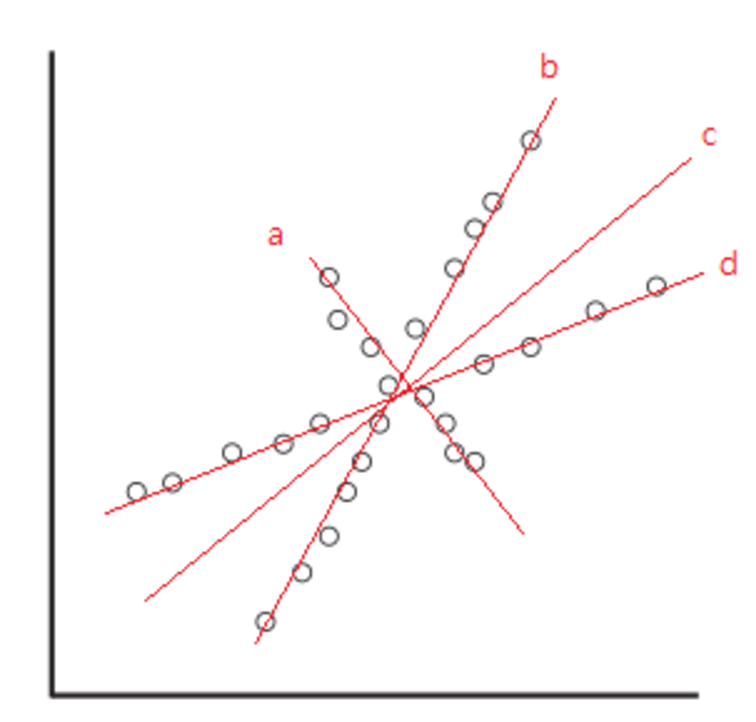
\includegraphics[width=0.5\linewidth]{figures/pca1.png}
    \end{figure}
    
\item \textbf{[2pts]} What will be its first principal component? %Options are given in the form of (first Principal Component, second Principal Component).
    \textbf{Select one:}
    \begin{list}{}
        %\item $\circle$ (a,b)
        \item $\circle$ d %(d,b)
        \item $\circle$ b %(b,d)
        \item $\circle$ c %(c,a)
        \item $\circle$ a %(a,c)
        
    \end{list}
    
    \item \textbf{[2pts]} \textbf{NOTE : This is continued from the previous question.} What is the second principal component in the figure from the previous question? %Options are given in the form of (first Principal Component, second Principal Component).
    % \begin{figure}[H]
    % \centering
    % 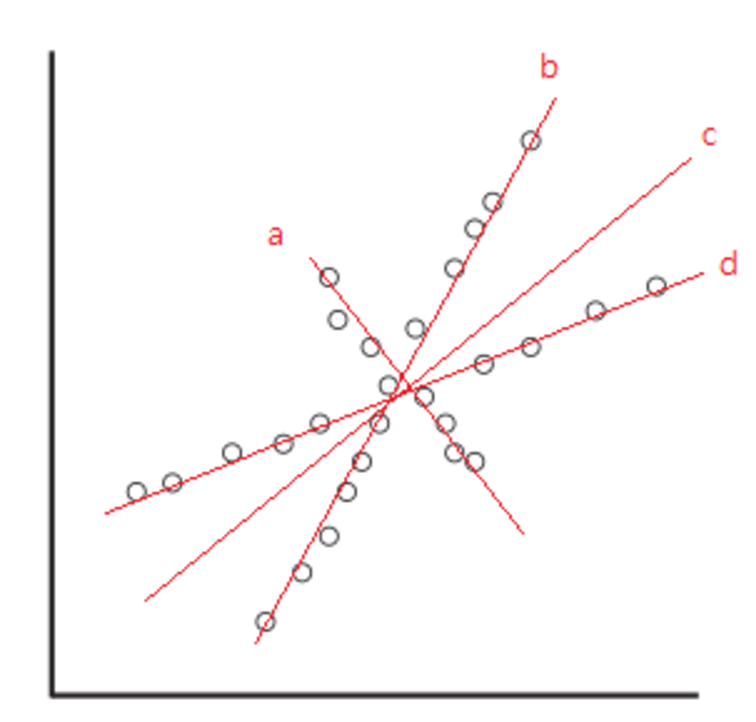
\includegraphics[width=0.65\linewidth]{figures/pca1.png}
    % \end{figure}
    \textbf{Select one:}
    \begin{list}{}
        %\item $\circle$ (a,b)
        \item $\circle$ d %(d,b)
        \item $\circle$ b %(b,d)
        \item $\circle$ c %(c,a)
        \item $\circle$ a %(a,c)
        
    \end{list}
    \item \textbf{[2pts]} \textbf{NOTE : This is continued from the previous question.}
What is the third principal component in the figure from the previous question?
     \textbf{Select one:}
    \begin{list}{}
        \item $\circle$ a
        \item $\circle$ b
        \item $\circle$ c
        \item $\circle$ d
        \item $\circle$ None of the above
        
    \end{list}

\end{enumerate}
\clearpage